\documentclass[10pt]{beamer}
% \documentclass[handout,10pt]{beamer}
\usepackage{my_style}
%%%%%%%%%%%%%%%%%%%%%%%%%%%%%%%%%%%%%%%%%%%%%%%%%%%%%%%%%%%%%%%%%%%%%%%%
%%%%%%%%%%%%%%%%%%%%%%%%%%%%%%%%%%%%%%%%%%%%%%%%%%%%%%%%%%%%%%%%%%%%%%%%
\title[Math/CS 375]{Lecture 02 - B}
\subtitle{\S 1.3 Floating-Point Errors}
\date{}

\begin{document}
% -------------------------------------------------
\begin{frame}
  \titlepage
\end{frame}
% -------------------------------------------------
\begin{frame}{Goals}

We will answer these questions:\\[3mm]
\begin{itemize}
    \item What is overflow, underflow, and demormalization? 
    
    \item What is the significance of machine epsilon? 
    
    \item How does arithmetic on the computer work, and what do we need to be wary of?

    \item How many significant digits do computational variables have? 

    \item How might significant digits be lost?
\end{itemize}
    
\end{frame}


\sectionframe{Overflow and Underflow}

% -------------------------------------------------
\begin{frame}{IEEE Double}

{\define{IEE Double Precision Float (FP64)}{
The \textbf{double precision float} has the form
\begin{equation*}
  x = \pm q \times 2^m.
\end{equation*}
It occupies 64 bits of memory. It is a specific standard format set by IEEE 755.  
}}
\begin{center}
  \pgfimage[width=8cm]{figs/ieee_double}
\end{center}

\question{What do the largest and smallest numbers look like?}

\end{frame}

% -------------------------

\begin{frame}[shrink]{FP64 Special Bit Sequences}
\begin{block}{Four Cases}
\begin{itemize}
  \item \textbf{Biggest finite number (realmax):}  
  \[
  \underbrace{0}_{\text{sign}}
  \;|\;
  \underbrace{11111111110}_{\text{exponent}}
  \;|\;
  \underbrace{1111\dots1111}_{52 \text{ ones}}
  \;\approx\; 1.7977\times 10^{308}
  \]

  \item \textbf{Smallest normalized number (realmin):}  
  \[
  \underbrace{0}_{\text{sign}}
  \;|\;
  \underbrace{00000000001}_{\text{exponent}}
  \;|\;
  \underbrace{0000\dots0000}_{52 \text{ zeros}}
  \;\approx\; 2.2251\times 10^{-308}
  \]

  \item \textbf{Signed Zero:}  
  \[
  \boxed{\pm}\;|\underbrace{\;00000000000\;|\;0000\dots0000}_{\text{all zeros}}
  \;=\;
  \pm0
  \]

  \item \textbf{Signed Infinity:}  
  \[
  \boxed{\pm}
  \;|\;
  \underbrace{11111111111}_{\text{all ones}}
  \;|\;
  \underbrace{0000\dots0000}_{52 \text{ zeros}} \;=\; \pm \infty
  \]

\end{itemize}
\end{block}

\end{frame}


% -------------------------------------------------
\begin{frame}[fragile]{Range}
\begin{center}
    
\begin{tabular}{l|c|c}
type    & range                                                     & approx
range\\\hline\hline
        & $-3.40\times 10^{38} \leq x \leq -1.18 \times 10^{-38}$   & \\
single  & 0                                                         & $2^{-126}\rightarrow 2^{128}$\\
        & $1.18 \times 10^{-38} \leq x \leq 3.40 \times 10^{38}$    & \\\hline
        & $-1.80\times 10^{308} \leq x \leq -2.23 \times 10^{-308}$ & \\
double  & 0                                                         & $2^{-1022}\rightarrow 2^{1024}$\\
        & $2.23 \times 10^{-308} \leq x \leq 1.80 \times 10^{308} $ & \\
\end{tabular}
\end{center}
\begin{lstlisting}
>> realmax
ans = 1.7977e+308

>> realmin
ans = 2.2251e-308
\end{lstlisting}
\question{What happens when you try to go beyond \texttt{realmax} or below \texttt{realmin}?}
\end{frame}
% -------------------------------------------------
% -------------------------------------------------
\begin{frame}{Overflow}

\begin{center}
\pgfimage[width=0.9\textwidth]{figs/floatingpoints}
\end{center}

\begin{itemize}

    \item \textbf{Overflow}:  
    When a computation produces a value larger than \texttt{realmax},  
    \[
    x > \texttt{realmax} \quad \Longrightarrow \quad \mathrm{fl}(x) = \infty.
    \]
\end{itemize}

\end{frame}

\begin{frame}{Underflow and Denormalization}

\begin{center}
\pgfimage[width=0.7\textwidth]{figs/floatingpoints}
\end{center}

\begin{itemize}
    \item \textbf{Underflow}:  
    When a value is too small 
    \[
    0 < |x| < \texttt{realmin},
    \]
    then it may round down to \underline{0 OR \textit{denormalize}}.
    \item \textbf{Denormalization}: The hidden bit becomes 0, allowing $x$ to be have representable numbers below \texttt{realmin}.
\end{itemize}

\end{frame}
% -------------------------------------------------
\begin{frame}[fragile]{Matlab Examples}
\begin{itemize}

\item Overflow - number is set to "infinity" 
\begin{lstlisting}
>> realmax*realmax
ans = Inf
\end{lstlisting}

\item Underflow to zero
\begin{lstlisting}
>> realmin*realmin 
ans = 0
\end{lstlisting}

\item Denormalization below \texttt{realmin}
\begin{lstlisting}
>> realmin/2
ans = 1.1125e-308 % not zero

>> realmin/256
ans = 8.6917e-311 % still not zero

>> realmin/2^53
ans = 0           % finally it's zero
\end{lstlisting}

\end{itemize}
\end{frame}



% -----------------------------------------------
\sectionframe{Machine Epsilon}
% -----------------------------------------------
%%%%%%%%%%%%%%%%%%%%%%%%%%%%%%%%%%%%%%%%%%%
\begin{frame}{The Additive Identity}

\question{
What happens when we add zero to a number $x$?
}


\onslide<2->{
\[
x+0=x
\]

\vfill
You get the same number $x$. Zero is called the additive identity.
}

\vfill

\onslide<3->{
\question{
If $x+\epsilon=x$, then what is $\epsilon$?
}
}

\end{frame}


\begin{frame}{Adding Floating-Point Numbers}

\begin{block}{Procedure}
    \begin{enumerate}
        \item Match the exponent of the smaller number to the larger number
        \item Align the binary points
        \item Add from right to left
    \end{enumerate}
\end{block}

\begin{example}
Add
\[
x_1 = 1.11011\times 2^{1},
\qquad
x_2 = 1.00111\times 2^{-2}.
\]
\end{example}

\begin{itemize}
    \item First, match the exponents:
    \[
    x_2
    =1.00111\times2^{-2}
    =0.00100111\times2^1.
    \]

    \item Now the significands can be added:
    \[
    \begin{array}{r}
      \phantom{+}1.11011000 \times 2^{1} \\
      \underline{+0.00100111 \times 2^{1}} \\
      \phantom{+}1.11111111 \times 2^{1}
    \end{array}
    \]
\end{itemize}

\end{frame}

\begin{frame}{Limited Storage}

We found the exact sum
\[
x_1+x_2 = 1.11111111\times2^1.
\]

\vfill

\begin{itemize}
    \item Suppose our floating-point system only stores
          \textbf{5 binary digits}.

    \item The exact answer does not fit:
    \[
    1.11111\underbrace{111}_{\text{cannot store}}\times2^1.
    \]

    \item If we truncate to 5 digits,
    \[
    \mathrm{fl}(x_1+x_2)
    =
    1.11111\times2^1.
    \]
\end{itemize}

\vfill

\keyidea{
Even if $x_1$ and $x_2$ can be stored exactly, their sum may not be
representable exactly in the same floating-point system.
}

\end{frame}


% \begin{frame}{Adding Floats}
% \begin{block}{Procedure}
%     \begin{enumerate}
%         \item Match the power of lower float to the higher float
%         \item Align the floats at the decimal
%         \item Add each digit from right to left (carry a one if necessary)
%         \item Truncate mantissa (if necessary)
%     \end{enumerate}
% \end{block}
% \begin{itemize}
%     \item Let $x_1  = 1.11011\times 2^{1} $
%     \item Let $x_2  = 1.00111\times 2^{-2}$ 
%     $$
%         \begin{array}{c}
%           \phantom{+}1.11011\phantom{001} \times 2^{1} \\
%         \underline{+0.00100111} \times 2^{1} \\
%                 \phantom{+}1.11111111 \times 2^{1}\\
%         \end{array}
%     $$
% \end{itemize}

% Since the original numbers only have digits of precision, we may also want to truncate the sum
% $$\mathrm{fl}(x_1 + x_2) = \mathrm{fl}(1.11111\underbrace{111}_{\text{truncate}} \times 2^1) = 1.11111 \times 2^1$$

% \end{frame}

% -------------------------------------------------

\begin{frame}{Adding in FP64}
\begin{example}
    
What happens when you add $x_1 = 1$ and $x_2 = 1/8$ in FP64? What does the bit sequence look like?
\end{example}
\begin{itemize}
    \item Let $x_1  = (1.0)_2\times 2^{0} $
    \item Let $x_2  = 1/8 = (1.0)_2\times 2^{-3}$ 
    \item $x_1 + x_2 = $
    $$
        \begin{array}{c}
          \phantom{+}1.000\phantom{} \times 2^{0} \\
        \underline{+0.001} \times 2^{0} \\
                \phantom{+}1.001 \times 2^{0}\\
        \end{array}
    $$
    \item $x_1 + x_2$ as a bit sequence
\end{itemize}
\begin{center} 
\begin{tabular}{|c||c|c|c|c|c|c|c|c|c|c|c||c|c|} 
   \multicolumn{1}{c}{Hidden} & \multicolumn{4}{l}{ } & \multicolumn{8}{l}{ } \\ 
   \multicolumn{1}{c}{bit} & \multicolumn{4}{l}{ } & \multicolumn{8}{l}{ } \\ 
\multicolumn{1}{c}{$\downarrow$} & \multicolumn{11}{l}
{$\leftarrow$ \hfill 52 bits \hfill $\rightarrow$} \\
\hline
 1 & 0 & 0 & 1 & 0 & 0 & 0 & 0 & 0 & 0 & 0 & 0 & e & e  \\ \hline 
\end{tabular} 
\end{center}
\end{frame}
% -------------------------------------------------
\begin{frame}{$\epsilon_m$ -- Machine epsilon}

\begin{example}
What happens when you add $x_1 = 1$ and $x_2 = 2^{-53}$ in FP64?
\end{example}

Let's start gradually\ldots Add $1/2$, $1/4, 1/8,$ and so on:
\begin{center} 
\begin{tabular}{|c||c|c|c|c|c|c|c|c|c|c|c||c|c|} 
   \multicolumn{1}{c}{Hidden} & \multicolumn{4}{l}{ } & \multicolumn{8}{l}{ } \\ 
   \multicolumn{1}{c}{bit} & \multicolumn{4}{l}{ } & \multicolumn{8}{l}{ } \\ 
\multicolumn{1}{c}{$\downarrow$} & \multicolumn{11}{l}
{$\leftarrow$ \hfill 52 bits \hfill $\rightarrow$} \\
\hline
 1 & 1 & 0 & 0 & 0 & 0 & 0 & 0 & 0 & 0 & 0 & 0 & e & e  \\ \hline \hline  
 1 & 0 & 1 & 0 & 0 & 0 & 0 & 0 & 0 & 0 & 0 & 0 & e & e  \\ \hline \hline  
 1 & 0 & 0 & 1 & 0 & 0 & 0 & 0 & 0 & 0 & 0 & 0 & e & e  \\ \hline  
\multicolumn{13}{c}{....... } \\ \hline 
 1 & 0 & 0 & 0 & 0 & 0 & 0 & 0 & 0 & 0 & 0 & 1 & e & e  \\ \hline \hline  
 1 & 0 & 0 & 0 & 0 & 0 & 0 & 0 & 0 & 0 & 0 & 0 & e & e  \\ \hline  
\end{tabular} 
\end{center}
\begin{itemize}
  \item $2^{-53}$ doesn't fit in the mantissa! 
  \item $\mathrm{fl}(1+2^{-52}) \ne 1$, but $\mathrm{fl}(1+2^{-53}) = 1$
\end{itemize}
\end{frame}
% -------------------------------------------------

\begin{frame}{}
\frametitle{$\epsilon_m$ -- Machine epsilon}
\begin{center}
    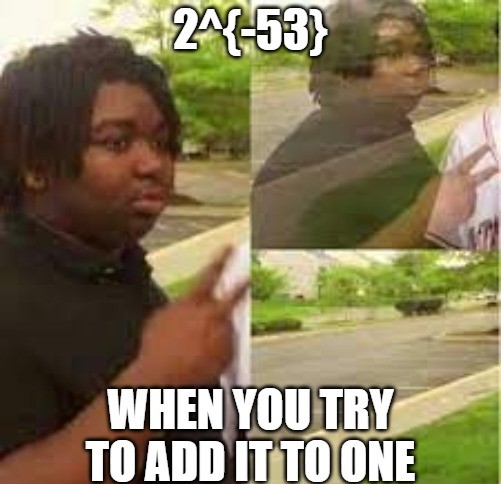
\includegraphics[scale=0.4]{figs/meme-epsilon.jpg}
\end{center}
\keyidea{Adding $1+2^{-53}$ in Matlab results in $1$. The quantity $\epsilon_m=2^{-52}$ is the cutoff.}
\end{frame}

% -------------------------------------------------
\begin{frame}{Importance}

    \begin{block}{In Math}
    If
    $$
    x+\epsilon = x
    $$
    then $\epsilon$ \textbf{must be the additive identity}, a.k.a. zero.
    \end{block}
    \vfill 

    \begin{block}{On Computers}
    Even if
    $$
    \mathrm{fl}(x+\epsilon) = x,
    $$
    $\epsilon$ may be \textbf{non-zero}. This is very bad!
    \end{block}

\keyidea{Machine epsilon is the limit at which math breaks down.}

    
\end{frame}

% -------------------------------------------------

\begin{frame}[fragile]{$\epsilon_m$ -- Machine epsilon}

{\define{Machine Epsilon}{
The \textbf{machine epsilon }$\epsilon_m$ is the smallest number such that
\begin{equation*}
  \mathrm{fl}(1+\epsilon_m) \ne 1,
\end{equation*}
where $\mathrm{fl}(x)$ represents the floating point representation of $x$.
}}
\begin{itemize}
  
  \item In English, 
    \begin{center}
    ``\textit{Machine epsilon is the smallest number that can be added to 1 without being lost to rounding.}"
    \end{center}
    \vspace{3mm}
    
  \item For FP32:  $\epsilon_m=2^{-23} \approx10^{-7} $.  
  \item For FP64:  $\epsilon_m=2^{-52} \approx 10^{-16}$.  

\end{itemize}

\end{frame}
% -------------------------------------------------
\begin{frame}[fragile]{Machine epsilon in Matlab}
\begin{itemize}
    \item \texttt{eps} is a built-in variable 
\begin{lstlisting}
>> eps
ans = 2.2204e-16

>> eps('single')
ans = 1.1921e-07
\end{lstlisting}

\item The following demonstrate machine epsilon rounding error
\begin{lstlisting}
>> 1+eps == 1+eps % this is fine 
ans = 1

>> 1+eps == 1 % this is fine 
ans = 0

>> 1+eps/2 == 1 % trouble 
ans = 1

>> 2+eps == 2 % trouble 
ans = 1
\end{lstlisting}
\end{itemize}
\end{frame}


\begin{frame}[fragile]{Rounding Problem}

\begin{example}
    What is the smallest number $a$ such that $\mathrm{fl}(a+32) \ne 32$ in FP64?
\end{example}

\begin{itemize}

  \item $a$ is so small relative to 32 that just barely avoids rounding
  \item Some use the notation $a = \epsilon(32)$ to describe the number $a$
    $$
    \epsilon(32)  = \epsilon_m \cdot |32| = 2^{-52} \cdot |x|
    $$
  \item Since $32 = 2^5$
    $$
    a < 2^{-52} \cdot 32 = \frac{2^5}{2^{52}} = 2^{-47} \approx 7.1\times10^{-15}
    $$

    \item You can also do this in Matlab 
\begin{lstlisting}
>> eps(32)
ans = 7.1054e-15
>> 32 + eps(32) == 32 % false, eps(32) is not rounded off
\end{lstlisting}
\end{itemize}

\end{frame}

 % -------------------------------------------------
\sectionframe{Floating Point Rules}
 % -------------------------------------------------

\begin{frame}{Review Error}
\define{Absolute Error}{
\textbf{Absolute error}, or usually just \textbf{error}, is
\begin{align*}
\text{Error}(x_a) &= |x_t - x_a| = |\text{true value} - \text{approximate value}|
\end{align*}
} 

\define{Relative Error}{
\textbf{Relative error} is
\begin{align*}
\text{Rel}(x_a) &= \left|\frac{x_t - x_a}{x_t}\right| = \left|\frac{\text{true value} - \text{approximate value}}{\text{true
value}}\right|
\end{align*}
}

\define{Percentage Error}{
\textbf{Percentage error} is
\begin{align*}
\left|\frac{x_t - x_a}{x_t}\right|\times 100 \% = \left|\frac{\text{true value} - \text{approximate value}}{\text{true
value}}\right| \times 100 \%
\end{align*}
}

\end{frame}

% -------------------------------------------------
\begin{frame}{Floating Point Rules}
\begin{block}{Rule 1.} 

\[\mathrm{fl}(x) = x (1 + \epsilon), \quad \mbox{where} \quad 
|\epsilon| < \epsilon_m\]
\end{block}

\begin{block}{Rule 2.} 
For all operations $\odot$ (one of $+, -, *, / $)

\[\mathrm{fl}(x \odot y ) = (x \odot y) 
(1 + \epsilon_{\odot} ), \quad \mbox{where} \quad 
|\epsilon_\odot | < \epsilon_m\]
\end{block}

\begin{block}{Rule 3.}
For $+, *$  operations \[\mathrm{fl}(a \odot b) = \mathrm{fl}(b \odot a)\]
\end{block}

There were many discussions on what conditions/ rules
should be satisfied by floating point arithmetic. 
The IEEE standard is a set of standards adopted by many
CPU manufacturers.
\end{frame}
% -------------------------------------------------

\begin{frame}{Relative Error for Floats}

\begin{itemize}
    \item The number $x\in \mathbb{R}$ stored as FP64 is 
    $$ \mathrm{fl}(x) = \underbrace{x}_{\text{the number}} \underbrace{(1+\epsilon)}_{\text{close to 1}}$$
    where $|\epsilon| \le 2^{-52}$

    \item We can use the rule to find \textbf{relative error}
        \begin{align*}
            \mathrm{Rel}(x) &= \frac{| true - approx|}{|true|}\\ 
             &= \frac{| x - \mathrm{fl}(x)|}{|x|}\\ 
             &= \frac{| x - x(1+\epsilon)|}{|x|}\\  
              & = |  \epsilon| \le 2^{-52}
        \end{align*}
\end{itemize}
\end{frame}

% -------------------------------------------------
\begin{frame}{Absolute Error for Floats}
\begin{example}
    Use the floating point rules to find the \textbf{absolute error} between $x$ and fl$(x)$.
\end{example}

\begin{itemize}
    \item By rule 1, we have fl$(x)=x(1+\epsilon),$ where $|\epsilon|<\epsilon_m$.
    \item The absolute error is 
            \begin{align*}
            \mathrm{Rel}(x) &= {| true - approx|}\\ 
             &= {| x - \mathrm{fl}(x)|}\\ 
             &= | x - x(1+\epsilon)|\\  
              & = |  x\epsilon|\\
              &\le |x|\epsilon_m
        \end{align*}
    \item This calculation says that the error between $x$ and fl$(x)$ depends on the \textit{magnitude of $x$}
 \end{itemize}
\end{frame}
% -------------------------------------------------
\begin{frame}{Floating Point Arithmetic}

\question{
Consider adding the triple sum $y = a + b + c $ on the computer. How is this handled? 
What is the error?
}  

\bigskip
Done as $ \mathrm{fl}( \mathrm{fl}(a+b) + c) $
\begin{eqnarray*} 
\eta & = & \mathrm{fl}(a+b) = (a+b)(1+\epsilon_1) \\
y_1  & = & \mathrm{fl}( \eta+ c) =  (\eta+c)(1+\epsilon_2) \\
     & = & \left[ (a+b)(1+\epsilon_1)   +c \right] (1+\epsilon_2) \\ 
     & = & \left[ (a+b +c) + (a+b) \epsilon_1)  \right] (1+\epsilon_2) \\ 
     & = &  (a+b +c) \left[1 + \frac{a+b}{a+b+c} \epsilon_1
(1+\epsilon_2) + \epsilon_2
  \right]
\end{eqnarray*}

So disregarding the high order term $\epsilon_1 \epsilon_2 $ 
\[ \mathrm{fl}( \mathrm{fl}(a+b) + c) = (a+b+c) (1 + \epsilon_3) 
\quad \mbox{with} \quad \epsilon_3 \approx \frac{a+b}{a+b+c} \epsilon_1 +
\epsilon_2\]
\end{frame}
% -------------------------------------------------
\begin{frame}{Addition Error for Floats}

If we redid the computation as $ y_2 = \mathrm{fl}( a + \mathrm{fl}(b+c)) $
we would find 

\[
\mathrm{fl}( a + \mathrm{fl}(b+c)) = (a+b+c) (1 + \epsilon_4) 
\quad \mbox{with} \quad \epsilon_4 \approx \frac{b+c}{a+b+c} \epsilon_1
+ \epsilon_2\]

The first error is \underline{amplified} by the factor $(a+b)/y$ in the
   first case and $(b+c)/y$ in the second case. ($y = a+b+c$) 

\bigskip
\keyidea{
Order matters. To optimize accuracy, add numbers from least to greatest. However, sorting before adding is usually not worth the cost! 
}
\end{frame}

% -------------------------------------------------
\begin{frame}{Error from Exponentiation}

\question{
What happens to floating point error when we compute $x^n$?
}

\bigskip

On a computer, exponentiation is performed via repeated multiplication:
\[
x^n = \underbrace{x \cdot x \cdot \dots \cdot x}_{n-1 \text{ times}}
\]

Using the floating point rule for multiplication,
\[
\mathrm{fl}(x \cdot y) = (x y)(1+\epsilon), \quad |\epsilon| \le \epsilon_m
\]

\bigskip

Each multiplication introduces a small relative error.
After $n-1$ multiplications, the computed result is
\[
\mathrm{fl}(x^n) = x^n (1+\epsilon_1)(1+\epsilon_2)\cdots(1+\epsilon_{n-1})
\]

\end{frame}

% -------------------------------------------------
\begin{frame}{Error Growth in Powers}

Ignoring higher-order terms (products of $\epsilon_i$),
\[
(1+\epsilon_1)(1+\epsilon_2)\cdots(1+\epsilon_{n-1})
\;\approx\;
1 + (\epsilon_1 + \epsilon_2 + \cdots + \epsilon_{n-1})
\]

Therefore,
\[
\mathrm{fl}(x^n) = x^n (1 + \epsilon_n),
\quad
|\epsilon_n| \lesssim (n-1)\epsilon_m
\]

\bigskip

\begin{itemize}
    \item Relative error grows \textbf{linearly} with the exponent
    \item Large powers magnify rounding error
    \item This effect appears even if $|x| \approx 1$
\end{itemize}

\bigskip

\keyidea{
Repeated operations accumulate error.
Exponentiation amplifies floating point error as the power increases.
}

\end{frame}

% -------------------------------------------------

\sectionframe{Significant Digits}

% -------------------------------------------------
\begin{frame}{Significant Digits}

\define{Significant Digits}{
\textbf{Significant digits} are digits in a number justified by the accuracy of the means of measurement. 
}
\bigskip

Example: Measurement from a ruler which goes from 0.0 to 9.0 (in cm):  
\begin{itemize}
\item $x=.23 \times 10^{1}cm$
\item two significant digits
\item 2 is the most significant digit
\item 3 is the least significant digit
\end{itemize}
\bigskip
\begin{itemize}
\item $x=.40 \times 10^{1}cm$
\item still two significant digits
\end{itemize}
\bigskip
\begin{itemize}
\item $x=.400 \times 10^{1}cm$
\item  The last zero is meaningless. From now on, we will never write it
\end{itemize}
\end{frame}
% -------------------------------------------------
\begin{frame}{Why it Matters}
    \begin{figure}
        \centering
        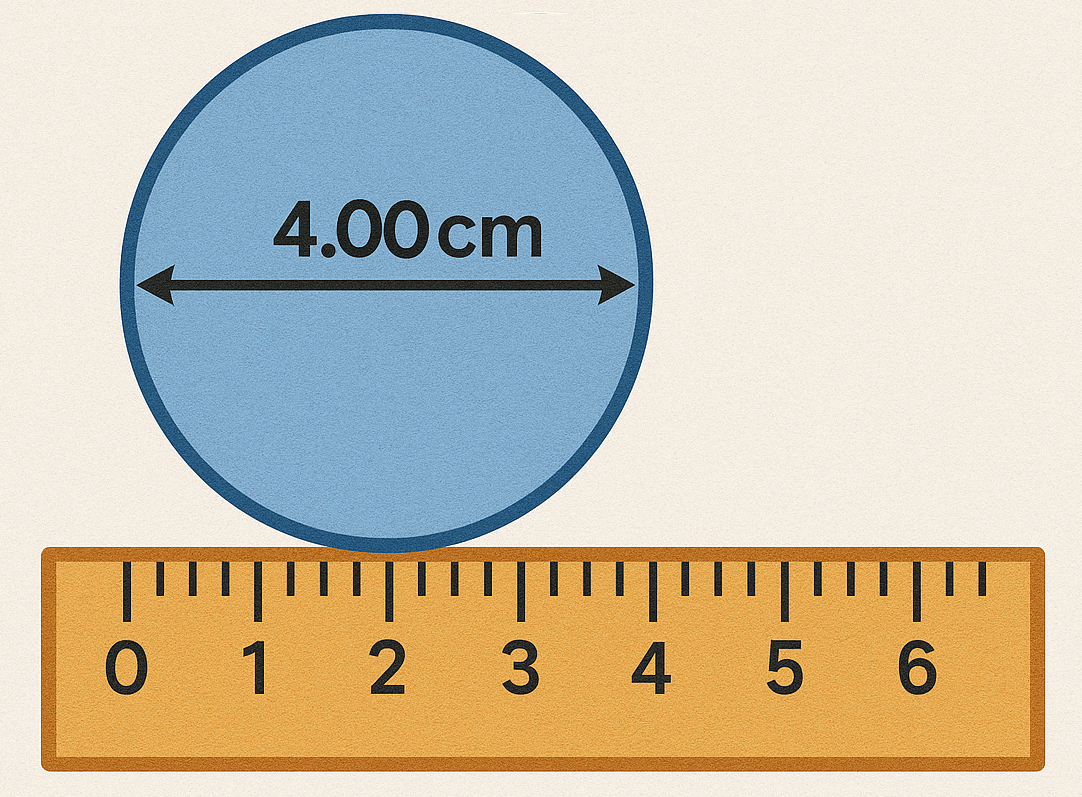
\includegraphics[width=0.3\linewidth]{figs/measure.png}
    \end{figure}
    \begin{itemize} 
        \item You measure the diameter to be 4.00 cm with 3 significant digits. 
        \item Then the area of the circle would be 
            \begin{align*}
                A &= \pi (D/2)^2\\
                  &= \pi (4.00/2)^2\\
                  & \approx 12.566370614359172
            \end{align*}
        \keyidea{
        \begin{itemize}
            \item We \textbf{cannot} report $A=$12.566370614359172 
            \item We must report 3 significant digits $A \approx 0.126 \times 10^2 \;\;  \text{cm}^2$
        \end{itemize}

        
        } 
    \end{itemize}
    
\end{frame}
% -------------------------------------------------
\begin{frame}{Significant Digits}
\begin{center}
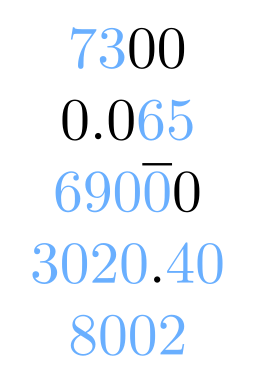
\includegraphics[scale=0.5]{figs/SigFigs.svg.png}
\end{center}
\begin{itemize}
    \item There are several rules to counting significant digits
    \item Digits in light blue are significant figures; those in black are not.
\end{itemize}
\end{frame}
% -------------------------------------------------
\begin{frame}{Precision/Significance}

{
\define{Precision}{
The \textbf{degree of precision} or \textbf{significance} of a floating point number is the number of significant digits it contains. 
}
}

\vspace{0.5cm}

In normalized form, it is easy to count precision 

\begin{itemize}
    \item $0.\underbrace{12345}_{\text{5 digits}}0000$
    
    \item $0.\underbrace{3700004}_{\text{7 digits}}0\times 10^4$
    
    \item $(0.\underbrace{10101010101}_{\text{11 digits or 11 bits}})_2\times 2^9$

\end{itemize}
\end{frame}

% -------------------------------------------------
\begin{frame}{Significant Digits in Floating Point Numbers}

\begin{itemize}
  \item Depends on the number of bits in the \textbf{mantissa}.
  \item Rule of thumb:
  $$
    \text{significant digits} =-\log_{10}(\epsilon_m)
  $$
\end{itemize}

\vspace{3mm}
\begin{center}
\begin{tabular}{|c|c|c|c|}
\hline
\textbf{Format} & \textbf{Mantissa Bits} & \textbf{Approx. Digits} & \textbf{Machine Epsilon} \\
\hline
Single (FP32)   & 23    & $\sim$7    & $2^{-23} \approx 1.19\times10^{-7}$ \\
Double (FP64)   & 52    & $\sim$15–16 & $2^{-52} \approx 2.22\times10^{-16}$ \\
Quad (FP128)    & 112   & $\sim$34   & $2^{-112} \approx 1.93\times10^{-34}$ \\
\hline
\end{tabular}
\end{center}

\keyidea{
All variables created in FP64 begin with 15-16 significant digits.
}
\end{frame}


% -------------------------------------------------
\sectionframe{Loss of Significance}
% -------------------------------------------------
\begin{frame}{Error with Addition}

\begin{block}{Loss of Precision via Rounding}
When adding two floating-point numbers with very different
orders of magnitude, digits from the \textbf{smaller} number may be lost.
\end{block}

\begin{itemize}
    \item Suppose $a$ and $b$ each have 16 digits of precision:
    \begin{align*}
        a &= 0.xxxx\,xxxx\,xxxx\,xxxx \times 10^0,\\
        b &= 0.yyyy\,yyyy\,yyyy\,yyyy \times 10^{-8}.
    \end{align*}

    \item Before adding, we must match the exponents:
    \[
        b
        =
        0.0000\,0000\,yyyy\,yyyy
        \underbrace{yyyy\,yyyy}_{\text{digits lost}}
        \times 10^0.
    \]

    \item Therefore the computer effectively adds
    \[
    \begin{array}{r@{\;}l}
          &0.xxxx\,xxxx\,xxxx\,xxxx\\
        + &0.0000\,0000\,yyyy\,yyyy\\
        \hline
          &0.xxxx\,xxxx\,zzzz\,zzzz
    \end{array}
    \times 10^0.
    \]
\end{itemize}

% \keyidea{
% The last 8 digits of $b$ cannot affect the computed sum because
% they fall beyond the available precision.
% }

\end{frame}
% -------------------------------------------------
\begin{frame}{Error with Subtraction}
\begin{block}{Loss of precision via cancellation}
Subtracting $fl(a-b)$ can lead to large loss of significance if $a \approx b$.
\end{block}
\begin{itemize}
    \item  Example: let $a$ and $b$ be numbers with 16 significant digits 
\begin{align*}
  a=\; & 0.xxxx\,xxxx\,xxxx\,xxx1\\
  b=\; & 0.xxxx\,xxxx\,xxxx\,xxx0\\
\end{align*}
\item  Then $a-b$ yields \qquad
\begin{tabular}{c l l}
& $0.xxxx\,xxxx\,xxxx\,xxx1$& \\
$-$& $0.xxxx\,xxxx\,xxxx\,xxx0$\\\hline
=& $0.\underbrace{0000\,0000\,0000\,000}_{\text{not significant}}1$ & \\
\end{tabular}
\end{itemize}

\define{Catastrophic Cancellation}{
\textbf{Catastrophic cancellation} refers to a phenomenon that occurs when subtracting two nearly equal numbers results in a loss of significant digits
}

\end{frame}
% -------------------------------------------------


% -------------------------------------------------
% \begin{frame}{Loss of Significance}

% \begin{example}
%   $x = 0.37214\,48693$ and
%   $y = 0.37202\,14371$.  What is the relative error in $x-y$ in a
% computer with 5 decimal digits of accuracy?
% \end{example}

% \begin{itemize}
%     \item When calculating $x-y$ on the computer, the actual result is
%     $$\mathrm{fl}( \mathrm{fl}(x)-\mathrm{fl}(y))$$

%     \item Thus
% \begin{align*}
%   \frac{|x-y - (\bar{x}-\bar{y})|}{|x-y|} 
% & = \frac{|0.37214\,48693 - 0.37202\,14371 - 0.37214 +
% 0.37202|}{|0.37214\,48693 - 0.37202\,14371|}\\
% & \approx 3\times 10^{-2}\\
% \end{align*}
%     \item Relative error is 3\%
% \end{itemize}
% \end{frame}
% -------------------------------------------------
\begin{frame}{Loss of Precision Theorem}

\begin{theorem}
    
Let $x$ and $y$ be (normalized) floating point machine numbers with
$x>y>0$.
\bigskip

If $2^{-p} \,\leq\, 1-\frac{y}{x} \,\leq\, 2^{-q}$ for positive integers $p$
and $q$, the significant binary digits lost in calculating $x-y$ is between $q$ and $p$.
Note: $q < p$
\end{theorem}

\bigskip 
\textbf{How to use:}
\begin{itemize}
    \item Calculate $f = 1-y/x$.
    \item $\log_2(f)$ gives number of lost binary digits 
    \item $\log_{10}(f)$ gives number of lost significant digits
\vspace{5mm}
    \item Note: you can't take the log of a negative number so 1-x/y won't work
    \item Tip: memorize $f = 1-\frac{small}{big}$
    

\end{itemize}
\end{frame}
% -------------------------------------------------
\begin{frame}{Loss of Precision Examples}
\begin{example}
  How many \underline{bits} are lost in the subtraction between $x=37.593621$ and $y=37.584216$?
\end{example}
\begin{equation*}
  2^{-12} \,<\, 1-\frac{y}{x} = 0.00025\,01754 \,<\, 2^{-11}
\end{equation*}
So we lose 11 or 12 bits in the computation of $x-y$.  yikes!
\begin{example}
How many \underline{significant digits} are lost in the subtraction between $x = 0.37214$ and
  $y = 0.37202$?
\end{example}
\begin{equation*}
  10^{-4} \,<\, 1-\frac{y}{x} = 0.00032 \,<\, 10^{-3}
\end{equation*}
   So we lose 3 or 4 digits in the computation of $x-y$.\\
Here, $x-y=0.00012$ which has only 1 or 2 significant digits.
\end{frame}
% -------------------------------------------------

\begin{frame}[fragile]{Quadratic Formula}

\begin{example}
Compute a root of the following equation: 
\[
x^2 + 2 p x - q = 0.
\] 
Let $p=10,000$ and $q=1$.
\end{example}

\begin{itemize}
    \item Quadratic formula $$ x = \frac{-b\pm \sqrt{b^2-4ac}}{2a}$$
    
    \item One of the roots can be computed with $$ y_1 = -p + \sqrt{p^2 + q}$$
    
\begin{lstlisting} 
>> p = 10000; q = 1;
>> y1 = -p+sqrt(p^2 + q) 
y1 = 5.000000055588316e-05  
\end{lstlisting} 

\end{itemize}
\end{frame}
% -------------------------------------------------
\begin{frame}[fragile]{Issue with Cancellation}

    \begin{itemize}
        \item To verify the accuracy of the solution $y_1$, we may substitute the value back into the equation 
            \[
            x^2 + 2 p x - q = 0.
            \] 
        \item We expect the value of $\epsilon_1$ to close to machine precision  
        \[
        \epsilon_1 = y_1^2 + 2 p y_1 - q 
        \] 
        \item However, it is \underline{8 orders of magnitude} away from $\epsilon_m$
\begin{lstlisting} 
>> p = 10000; q = 1;
>> y = -p+sqrt(p^2 + q) 
y1 = 5.000000055588316e-05  
>> y1^2 + 2*p*y1 - q  
ans = 1.361766321927860e-08
\end{lstlisting} 
        
    \end{itemize}
    
\end{frame}
% -------------------------------------------------
\begin{frame}{Conjugation}

\define{Conjugate}{
For the binomial $a+b$, is its \textbf{conjugate} is $a-b$.
}

\begin{itemize}
    \item When you multiply two conjugates, you always $(a+b)(a-b) = a^2 - b^2$
    \item When calculating $a-b$, we may employ the \textbf{conjugation method}:
        $$a-b = (a-b)\frac{a+b}{a+b} = \frac{a^2-b^2}{a+b} $$
    \item This is particularly useful for the quadratic formula 
        $$ x = \frac{-b + \sqrt{b^2-4ac}}{2a} $$

\end{itemize}


\end{frame}
% -------------------------------------------------
% \begin{frame}[fragile]
% \frametitle{Comparing the two methods}
% \begin{minipage}[t]{4.2in} 
% Algorithm 1 finds root with $y = -p + \sqrt{p^2 + q} $
% \begin{lstlisting}[mathescape]
% $ s $  := $ p^2$       
% $ t $  := $  s+ q $    
% $ u $  := $  \sqrt{t}$
% $ y $  := $ -p + u $ 
% \end{lstlisting}
% \end{minipage} 
% \bigskip


% \begin{minipage}[t]{4.2in} 
% Algorithm 2 finds root with $y = \frac{ q }{  p + \sqrt{p^2 + q}} $
% \begin{lstlisting}[mathescape]
% $ s $  := $ p^2 $
% $ t $  := $ s+ q$
% $ u $  := $ \sqrt{t}$
% $ v $  := $ p+ u $
% $ y $  := $ q/v$
% \end{lstlisting}
% \end{minipage} 
% \smallskip

% $\Rightarrow$ Step 4 of Algorithm 1 can have severe cancellation when 
% $p >> q$ and when $p$ is positive. 
% \end{frame}
% -------------------------------------------------
\begin{frame}[fragile]{The Fix}
\begin{itemize}
    \item The two methods produce slightly different roots 
\begin{lstlisting} 
>> p = 10000; q = 1;
>> y1 = -p+sqrt(p^2 + q) % original method
y1 = 5.000000055588316e-05  

>> y2 = q/(p+sqrt(p^2+q)) % new formula with conjugation
y2 = 4.999999987500000e-05  
\end{lstlisting} 

\item The second formula has a much lower error
\begin{lstlisting} 
>> y1^2 + 2*p*y1 - q  % checking residue for method 1
ans = 1.361766321927860e-08

>> y2^2 + 2*p*y2 - q % checking residue for method 2 
ans = -1.110223024625157e-16
\end{lstlisting} 

\end{itemize}
\keyidea{First formula has an error on the order of $10^{-8}$ while the fixed formula has an error around $10^{-16}$.}
\end{frame}

\end{document}
